\section{Two targets without the volume term, and an honest error for the simpler one}
\label{sec:profile}

\subsection{The profile likelihood: unbiased score, curvature too sharp}

For amplitudes that enter linearly with known noise, the profile score is exactly unbiased
whatever the true amplitudes are (App.~\ref{app:sandwich}). The amplitudes are fixed unknowns, no
distribution is assumed for them, and nothing depends on the reference frequency. This is the
errors-in-variables model with known error covariance, for which the consistency of the slope is
classical; the classical caveat is that the variance of the estimator is not the inverse Fisher
information. In the notation of Eq.~(\ref{eq:JT}) the score variance is $\J + \Tm$ while the
curvature of $\tfrac12\chimin$ is $\J$, so the estimator has covariance
\begin{equation}
  \mathrm{Cov}(\hat\beta) = \J^{-1} (\J + \Tm)\, \J^{-1} ,
  \label{eq:sandwich}
\end{equation}
a sandwich \citep{huber1967,white1982} whose middle term is known in closed form here. An interval
built from the curvature of the profile likelihood, or from an MCMC chain run on
Eq.~(\ref{eq:Lprof}), is too narrow by
\begin{equation}
  \frac{\mathrm{sd}(\hat\beta)}{\sigma_{\rm curv}} = \sqrt{1 + \frac{\Tm}{\J}}
  = \sqrt{1 + \frac{\sum_p V_p}{\sum_p u_p V_p}} ,
  \label{eq:sdz}
\end{equation}
the second form for one region and one component. The ratio $\Tm/\J$ is the inverse of the
lever-arm-weighted mean squared signal-to-noise ratio of the amplitudes. For a region measured through
a few bright pixels it is negligible. For an index shared by many faint pixels it is not, however
well the index itself is measured: this is why the profile likelihood was found unbiased but ``up to
two times too narrow'' for a full-sky index at low signal to noise in our earlier simulations
(\exref{E017}), and why it is safe for the bright regions of the polarized sky (\exref{E036}).

\subsection{The error from one data set}

On real data $\J$ has to be evaluated at fitted amplitudes, and here is a trap. The fitted amplitudes
are the true ones plus noise with covariance $\A^{-1}$, and
\begin{equation}
  \E\big[\J(\hat a)\big] = \J + \Tm :
\end{equation}
the plug-in information estimates the score variance, not the curvature. A sandwich built as
$\J(\hat a)^{-1}[\J(\hat a) + \Tm]\J(\hat a)^{-1}$ is therefore narrower than the curvature width it
was meant to widen. The consistent estimate is
\begin{equation}
  \J_{\rm c} = \J(\hat a) - \Tm , \qquad \widehat{\mathrm{Cov}}(\hat\beta) = \J_{\rm c}^{-1}\, \J(\hat a)\, \J_{\rm c}^{-1} ,
  \label{eq:debiased}
\end{equation}
and a region for which $\J_{\rm c}$ is not positive has fitted amplitudes consistent with noise and no
measured index. Both $\J(\hat a)$ and $\Tm$ come from quantities already formed in the fit.

\begin{figure}
\centering
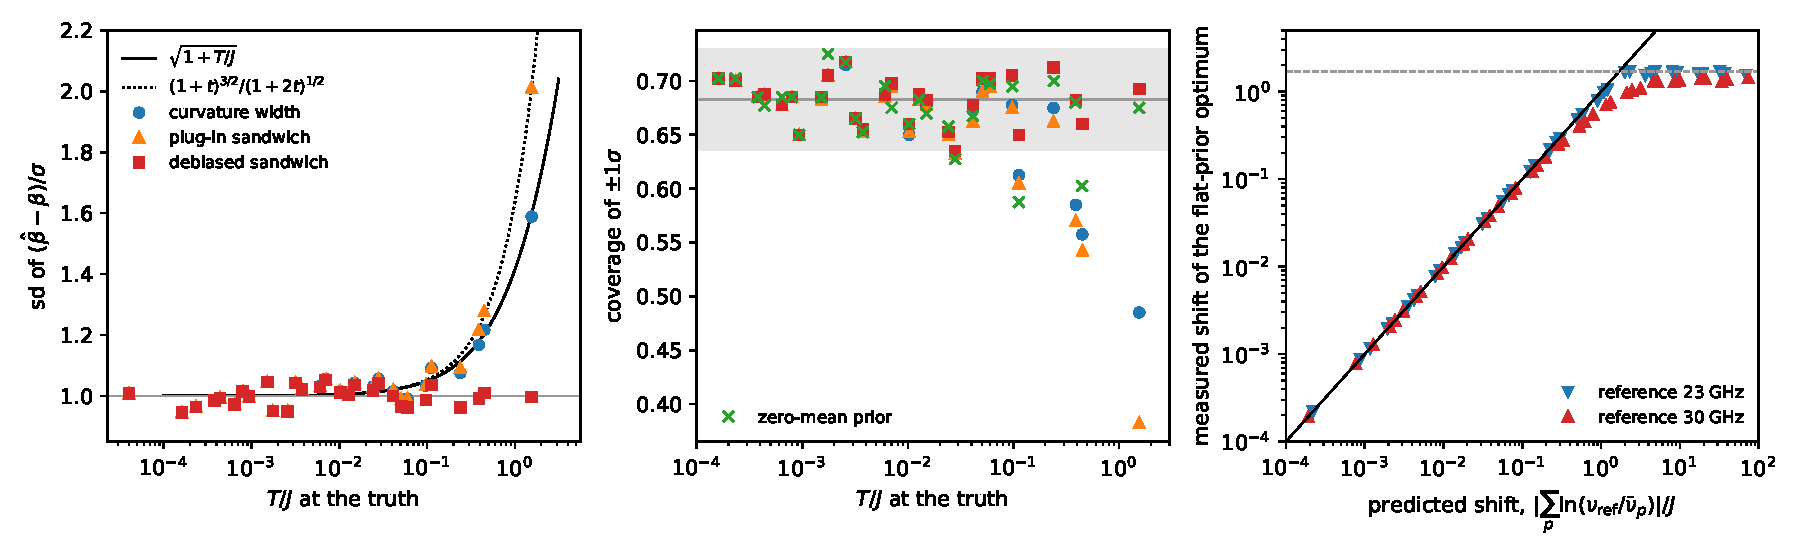
\includegraphics[width=\textwidth]{figures/fig_ladder.pdf}
\caption{One index shared by $n = 32$ to 8192 heavy-tailed amplitudes at five bands, per-amplitude
signal-to-noise ratio from 9 to 0.07, 400 noise realizations per cell; cells in which the index is
measured to better than 0.25 (\exref{E041}). Left: standard deviation of the standardized error of the
profile optimum with three error estimates, each taken from the same data set as the estimate, against
$\Tm/\J$ at the truth. The curvature width follows Eq.~(\ref{eq:sdz}) (line), the plug-in sandwich is
narrower still (dotted: its expected factor), and the debiased sandwich of Eq.~(\ref{eq:debiased})
stays at one. Centre: coverage of the $\pm1\sigma$ interval for the same three and for the zero-mean
prior; the band is $\pm2$ binomial standard errors around 0.683. Right: shift of the flat-prior
optimum from the profile optimum against the first-order prediction of Sect.~\ref{sec:flat}, at
references of 23 and 30 GHz, all 40 cells; the dashed line is the edge of the allowed range.}
\label{fig:ladder}
\end{figure}

Figure~\ref{fig:ladder} tests this over a ladder designed to reach the regime where it matters:
many faint amplitudes sharing one index, with predictions written down before the run
(\exref{E041}). With the curvature width the standard deviation of the standardized error equals
Eq.~(\ref{eq:sdz}) within 0.054 in all 30 cells where the index is measured, up to 1.59 at
$\Tm/\J = 1.56$, and 68 percent intervals cover the truth as rarely as 49 percent of the time. With
the plug-in sandwich they cover it 38 percent of the time. With Eq.~(\ref{eq:debiased}) the
standardized error has standard deviation 0.95 to 1.05 and the coverage is 0.65 to 0.72 in 29 cells
and 0.635 in one; the mean standardized error is within 0.10 everywhere. The coupled case with
several regions, three components and the dense WMAP covariances is tested in
Sect.~\ref{sec:data}.

\subsection{The zero-mean prior with a free scale}

The Bayesian relative of the profile likelihood is a zero-mean Gaussian amplitude prior with a
variance per index region that is inferred with the index. For a noise pattern that is common to the
amplitudes of a region, $w_{pb} = w_b$, the marginal likelihood depends on the data through
$q(\beta) = \sum_p b_p^2/A$ only, with $b_p = \sum_b w_b m_b d_{pb}$ and $A = \sum_b w_b m_b^2$, and
maximizing over $\tau$ gives
\begin{equation}
  \ln\mathcal{L}_{\tau}(\beta) = \tfrac12\, q(\beta) - \tfrac{n}{2}\ln q(\beta) + \mathrm{const}
  \qquad (q > n) ,
\end{equation}
a monotonic function of the profile log-likelihood $\tfrac12 q$. The optimum is the profile optimum,
and the curvature is the profile's times $1 - n/q$, which is the plug-in form of $1/(1+\Tm/\J)$. In
this case the zero-mean prior with a free scale \emph{is} the profile likelihood with its sandwich
width: the prior learns from the scatter of the fitted amplitudes how much of them is noise.
Simulation confirms the identity to the tolerance of the optimizer (\exref{E041}).

When the noise pattern varies between the amplitudes, as it does on real maps, the two estimators
part. The Gaussian prior is then a model for the amplitudes, real polarized amplitudes are far from
Gaussian, and the bright ones carry whatever noise pattern they happen to have. In the ladder the
resulting bias of the zero-mean prior is between $-0.6$ and $+0.3$ posterior standard deviations,
with a sign that belongs to the amplitude configuration and not to the noise level, while its
coverage stays within 0.59 to 0.73. On the realistic sky of Table~\ref{tab:flat} it was within 0.11
standard deviations except in one class at four times the real noise ($-0.30$; \exref{E036}). A scale
map in place of a single scale reduces it there. We therefore take the profile likelihood with the
debiased sandwich as the estimator of record and report the zero-mean prior beside it. What the
prior offers in exchange is a proper posterior, which a hierarchical model of an index field needs.

\subsection{What each target is good for}

\begin{table}
\centering
\caption{The index targets of Sect.~\ref{sec:model} for an index shared by many amplitudes, as
established by the experiments cited.}
\label{tab:targets}
\small
\begin{tabular}{p{3.2cm}p{3.6cm}p{3.6cm}p{4.2cm}}
\toprule
target & centre & width & depends on $\nuref$ \\
\midrule
flat-prior marginal (and Gibbs with flat amplitude priors) & shifted by
$\ln(\nuref/\nupiv)\,\sigma_1^2$ (\exref{E036}, \exref{E041}) & curvature & yes: tilt
$e^{n\beta\ln\nuref}$ \\
profile likelihood & unbiased (\exref{E036}, \exref{E041}) & curvature too narrow by
$\sqrt{1+\Tm/\J}$; debiased sandwich calibrated (\exref{E041}) & no \\
zero-mean prior, free scale per region & unbiased for a common noise pattern; up to 0.6 sd otherwise
(\exref{E041}) & calibrated where unbiased & no \\
re-solve move inside a Gibbs sweep & close to the profile optimum & too wide by $\sqrt{T}$,
Eq.~(\ref{eq:Tk}) (\exref{E035}) & no \\
\bottomrule
\end{tabular}
\end{table}

Table~\ref{tab:targets} collects the results. Two remarks on scope. First, for an index \emph{field}
with a hierarchical prior the profile likelihood is not enough at low signal to noise: the profile
maxima of faint regions scatter, and a hierarchy reads that scatter as field variance
(\exref{E012}). A proper amplitude prior is then needed, and its specification becomes part of the
model (Sect.~\ref{sec:limits}). Second, the statements above are for amplitudes that enter linearly
with known Gaussian noise. Beams, masks and a correlated-noise model that is itself uncertain change
the numbers, not the structure.
